\section*{Background}
In this section we explain some concepts we had to understand implementing our project. 

\subsection*{HTTP Protocol}
The Hypertext Transfer Protocol (HTTP) is an application layer protocol which defines how data can be exchanged over the Internet. It is generally sent over TCP, as it relies on a reliable transport protocol. 
As a client-server protocol, requests are initiated by the recipient (browser) and responses are served by the provider (web server). The structure of these requests and responses is defined by HTTP. \footnote{https://developer.mozilla.org/en-US/docs/Web/HTTP/Overview} For our project, we mainly focused on version HTTP 1.1. \\

The general structure of a request is the following: The first line denotes the \textbf{Method}, \textbf{Path} and \textbf{Version of the Protocol}. The following lines are called \textbf{Headers} and contain information for the servers. An empty line signals the end of the headers, for some request types (such as POST) the \textbf{Request Body} follows. A header to point out would be the \textbf{Connection} header, which was introduced in version 1.1 to provide persistent connections by reusing a TCP connection for multiple request/responses instead of opening a new connection for each response. The response follows the same structue, just that the first line contains the Version of the Protocol First, then the Status Code and Status Message \footnote{See HTTP Codes https://developer.mozilla.org/en-US/docs/Web/HTTP/Status} \\

There are several Request Methods which signal what kind of action should be performed. \footnote{https://datatracker.ietf.org/doc/html/rfc1945\#section-8} For example: 
\begin{description}
    \item[GET]retrieve state representation of target resource. Parameters sent through URL 
    \item[HEAD]retrieve only metadata. 
    \item[POST]request that target resource processes the representation in the request body. 
\end{description}

\begin{figure}[h]
	\centering
	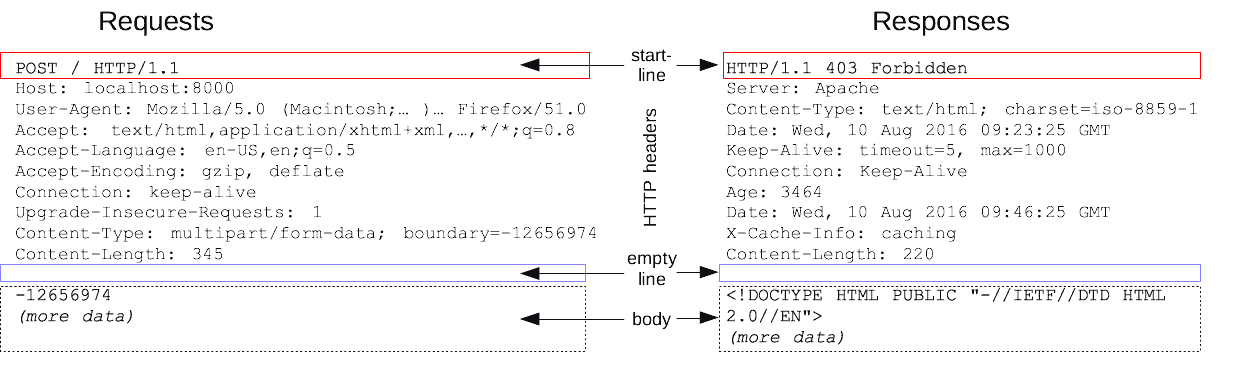
\includegraphics[width=0.9\textwidth]{figures/http_structure.png}
	\caption{HTTP Requests and Responses}
\end{figure} %QUELLE: https://developer.mozilla.org/en-US/docs/Web/HTTP/Messages

\subsection*{Common Gateway Interface}
The Common Gateway Interface (CGI) \footnote{https://datatracker.ietf.org/doc/html/rfc3875} is a technology we encountered during our research on handling HTTP POST requests. CGI is an interface that defines how the web server interacts with external programs. This enables the creation of dynamic content, such as generating user-specific webpages or processing form submissions, and facilitates communication between the web server and application backend services.

\begin{figure}[h]
	\centering
	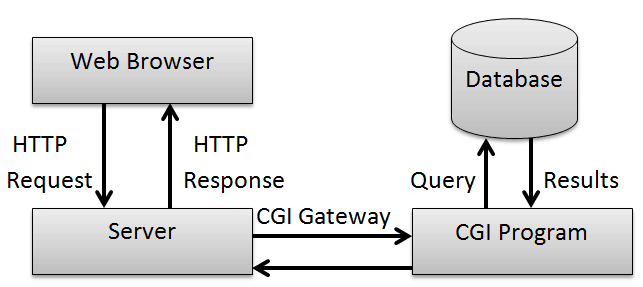
\includegraphics[width=\textwidth]{figures/Common-Gateway-Interface.png}
	\caption{The Common Gateway Interface}
\end{figure}

When a request with a URL denoting a CGI script, like example.com/backend.cgi, enters the web server, the server locates the executable file called backend.cgi. It then spawns a process to execute the CGI script and communicates with this process via piped standard input/output and environment variables. After the CGI script sends its response to the web server, the server may verify the response and forward it to the client.\\

Although CGI is now quite outdated and less frequently used due to the inefficiency of spawning a new process for each request, enhanced versions such as FastCGI or SCGI are widely used. These versions improve performance by spawning CGI scripts only once. In our project we implemented the original CGI specification from 1997.

